\documentclass{article}
\usepackage{graphicx}
\usepackage{forest}
\usepackage{tikz}
\usepackage{float}
\usepackage{subcaption}
\usepackage{hyperref}
\usetikzlibrary{fit}
\graphicspath{ {./images/} }
\begin{document}
\title{An Implementation of Hypersuccinct Trees}
\author{Christopher Pack, Alexander Auras, Nathanael Stöhr, Charbono Lonyem Tegomo}
\date{\today}
\maketitle

%ADJUST FIGURE PLACEMENTS WHEN TEXT IS DONE
%ADJUST FIGURE PLACEMENTS WHEN TEXT IS DONE
%ADJUST FIGURE PLACEMENTS WHEN TEXT IS DONE

\begin{abstract}
This document describes a practical implementation of hypersuccinct tree encodings for ordered trees in C++. The theory is based on the procedures described in \cite{farzanMunro} and \cite{universalSuccinct}. A special focus lies on a space-efficient real-world-encoding and support of constant-time queries. We show that both of these constraints can be fulfilled in a practically usable implementation and provide a C++-library, Python-interface and GUI to showcase our results. We also summarize our findings regarding a short theoretical and practical analysis of the time- and space-requirements of an example service which reads, parses and writes XML-Files.

\end{abstract}

\tableofcontents

\section{Introduction} \label{Introduction}
Data storage is and has always been a challenge for multiple reasons, with the two probably most frequently occurring problems being access time and size. The challenges these problems pose only increase with more complex access mechanisms and datastructures.\\
One possible solution is the more efficient usage of the given space by the introduction of hypersuccinct data structures. Succinct data structures store data in some kind of compressed format, at or around the information-theoretical lower limit, while still allowing the execution of queries in an acceptable timeframe.\\
While much work has already been done on the theoretical site of things, the implementation of more complex succinct datastructures is not as well established. In this paper we present our practical implementation of hypersuccinct trees in C++ as an example of a complex hypersuccinct data structure. The implementation should be space-efficient and still allow the execution of constant-time queries.\\
The theoretical basis for our implementation can be found in \cite{farzanMunro} and \cite{universalSuccinct}. While mainly a proof of concept, our library should also allow for easy extension and be usable as a solid basis-implementation of a hypersuccinct tree.

\section{The Tree covering Algorithm} \label{The Tree covering Algorithm}
To achieve the succinct encoding of the tree we follow the algorithm described by Farzan and Munro \cite{farzanMunro}. This algorithm has several steps. At first, the decomposition algorithm is used to divide the tree into several smaller subtrees of roughly equal size. These trees, called Minitrees, are then with the same algorithm further decomposed into even smaller subtrees, called Microtrees. The decomposed trees follow certain rules. Their nodes are disjoint, except they may have a common root node. Edges between them that do not share a common root node always end in the root node of the child tree and start from the root node of the parent tree, except for at most one edge in a subtree, that may start from any node in that tree and connect to the root of the child tree. We call this last special type of connection “dummy-interconnection”.\\
This allows to represent the interconnections of these subtrees with so called Fully Indexable Dictionaries (FIDs). Only the dummy interconnections need their own handling. For these, we create a new dummy node on the interconnecting edge and store its pointer explicitly. Since there can at most be one such interconnection for each tree, the amount of created dummy nodes for a tree with $n$ nodes is bound by $O(\log (n))$.\\
For the other types of interconnection, we distinguish between two types. Trees with type 1 interconnections share a common root node, while trees with type 2 interconnections are connected via an edge between their root nodes. With the FIDs and an additional vector we can represent both these interconnections. We create a FID for each root node. In the FID we store information about the child nodes of the root. This information allows us to identify which child nodes belong to a common tree. We use the additional vector, the Typevector (TV), to distinguish between interconnections of type 1 and type 2, by storing that information in 1 bit for each tree.\\
For each Minitree we store its index in the FIDs and the data about its Microtrees together with some auxiliary information which will be described later. The size of this data of all mini-trees is in $o(n)$ bits.

\begin{figure}[H]
\begin{tabular}{ |p{3.5cm}p{8cm}|} 
 \hline
 child($v$, $i$) & The $i$-th child of node $v$. \\
 childRank($v$) & The index of node $v$ as child of it's parent node. \\
 getParent($v$) & The parent node of node $v$. \\
 degree($v$) & The degree (number of children) of node $v$. \\
 subtreeSize($v$) & The size of the tree with node $v$ as root. \\
 depth($v$) &  The number of edges from the root to the node $v$. \\
 height($v$) & The number of edges from the node $v$ to the furthest leaf in it's subtree. \\
 leftmostLeaf($v$) & The leftmost leaf descendant of node $v$. \\
 rightmostLeaf($v$) & The rightmost leaf descendant of node $v$. \\
 leafSize($v$) & The number of leaf nodes in the subtree of node $v$. \\
 leafRank($v$) & The number of leaves before and including $v$. \\
 \hline
\end{tabular}
\caption{Queries of the Hypersuccinct Tree}
\label{2.1:table1}
\end{figure}

\subsection{Functions and Queries of the Hypersuccinct Tree} \label{Functions and Queries of the Hypersuccinct Tree}
To have a succinct data structure we have to be able to execute efficient query operations on our data. The auxiliary information stored for each Minitree is fundamental for that. In fact, the information we store allows us to execute many commonly needed query operations within $O(1)$ time. That means a lot of complex calculations are done upon creating the data and the results are then stored efficiently to be quickly available when asked for. \\

\section{Our Implementation} \label{Our Implementation}
This section is a short description of our implementation, which is made in C++.

\subsection{Goals of the Implementation} \label{Goals of the Implementation}
This library is mainly ment to provide some practical proof that the encoding offered by \cite{farzanMunro} and \cite{universalSuccinct} works in practice. Be mindful that our goal was to implement a succinctly encoded tree as described in \cite{farzanMunro}, with huffman encoding being the only part from \cite{universalSuccinct} impacting our project, therefore other changes described in \cite{universalSuccinct} are not part of this implementation.\\
This still results in a library that is ready for use in actual programs, so long as the limited implementation of functions actually suffices, and we discuss some of the shortcomings of this implementation in Section \ref{Complexity Benchmarks}. This library is meant to be open and further refining and adding functionality should be possible and would be appreciated.\\
The library offers basic functionality around the hypersuccinct tree encoding such as generating a hypersuccinct tree from an .xml file, saving an encoded tree to a file and reading encoded files. The hypersuccinct tree offers a variety of queries, all implemented with a time complexity of $O(1)$.

\subsection{External Libraries} \label{External Libraries}
We use four external libraries in our project.
The first one, called Irrxml \cite{irrXMLLink}, serves an implementation to read efficiently from an xml file. We use this library to generate a basic tree structure from xml files which is then used for our encoding.\\
We make use of a small library which provides an implementation of space efficient Fully Indexable Dictionaries \cite{universalSuccinct}, called succinct\_bv \cite{succinctBVLink}, which is implemented as described in \cite{succinctBV}.
This library is very lightweight and has been modified personally by us to suit our needs.\\
To increase the performance of our encoding process (see Section \ref{Factory Complexity}), we utilize a multithreading library called thread-pool \cite{threading}, to provide an efficient multithreading library.\\
Lastly, we utilise the googletest library \cite{googletestLink} for unit tests.

\section{Implementation in Depth} \label{Implementation in Depth}
We present our implementation in detail, and highlight issues we encountered during our implementation process and how we solved them.\\
\subsection{The Hypersuccinct Tree Class} \label{The Hypersuccinct Tree Class}
The Hypersuccinct Tree class implements the entire hypersuccinct tree encoding. It consists of a struct representing Minitrees and one representing the lookup table entries.
Both of these structs use plenty of bitvectors to store relevant data for queries.\\

Hypersuccinct Nodes:\\
Nodes within the Hypersuccinct Tree are identified as triplets, where the first value denotes the Minitree, the second the microtree and the third the node number within the Microtree.\\

\subsubsection{The FID and identifying Trees} \label{The FID and identifying Trees}
FIDs represent the interconnections between trees at their roots, their type 1 and type 2 connections \cite{farzanMunro}, together with a Type Vector that shows which kind of connection the tree has.
Due to the way they are being generated, the FIDs do not share indices with their respective trees, since trees can share roots, while onyl one FID is generated per each unique root. Because of this, it is possible that there are less FIDs than there are trees, and their indices are different. (i.e. it is possible for the Minitree with $id = 7$ to be in the FID with $id = 5$).
This necessitates an index conversion whenever the FID or the type vector is used. Doing this conversion at runtime would not be possible within $O(1)$, since it would be necessary to go through each FID and count the trees contained within it, for both type 0 and type 1 connections.
This is further complicated by taking into account the fact that each tree is actually accounted for in two different FIDs. Firstly in the FID of its own root as a type 0 connection (Top FID), and secondly in the FID of its parent as type 1 (Low FID). Trees below dummies however have no low FID, as they are not directly below the root of their parent tree.\\
\begin{figure}[h]
	\begin{tabular}{ |p{3.5cm}||p{0.5cm}|p{0.5cm}|p{0.5cm}|p{0.5cm}|p{0.5cm}|p{0.5cm}|p{0.5cm}|p{0.5cm}|  }
		 \hline
		 \multicolumn{9}{|c|}{Vector indices for Trees} \\
		 \hline
		 Minitree Number & 0 & 1& 2 & 3 & 4 & 5 & 6 & 7\\
		 Minitree Top FID& 0 & 1 & 2 & 3 & 4 & 5 & 6 & 6\\
		 Minitree Low FID& - & 0 & 0 & 2 & 2 & 3 & - & -\\
		 \hline
	\end{tabular}
\caption{Example Indices for Minitrees}
\label{fid:table1}
\end{figure}
\begin{figure}[h]
	\begin{tabular}{ |p{3.5cm}||p{1cm}|p{1cm}|p{1cm}|p{1cm}|p{1cm}|p{1cm}|p{1cm}|p{1cm}|  }
		 \hline
		 Bitvector & Bit 1 &Bit 2&Bit 3&Bit 4& Bit 5 &Bit 6&Bit 7&Bit 8\\
		 \hline
		 Minitree FID 0 & 1 & 1& 0 & 1 & 0 & 0 & 1 & 1\\
		 Minitree Typevector 0& 0 & 1 & - & 0 & - & - & 1 & 0\\
		 Minitree Numbers & 0 & 3 &  0 & 1 & 1 & 1 & 5 & 2\\
		 \hline
		 Minitree FID 1 & 1 & 0& 1 & 1 & 0 & 1 & 1 & 1\\
		 Minitree Typevector 1& 0 & - & 1 & 1 & - & 1 & 1 & 0\\
		 Minitree Numbers & 3 & 3 &  6 & 7 & 3 & 8 & 9 & 4\\
		 \hline
	\end{tabular}
\caption{FID, Typevector and corresponding trees}
\label{fid:table2}
\end{figure}
Another issue arises when trying to analyze the FID and Typevectors of the Hypersuccinct Tree. Identifying which tree is at which position within even a single FID is not trivial. As demonstrated in Figure \ref{fid:table2}, the second type 1 tree in the first FID has the id of $5$, because the FID of tree $3$ contains tree $4$ already as a type 0 tree, meaning correctly identifying Bit $7$ as tree $5$ requires analysis of the FID of tree $3$. Additionally, it is important to note that the FID with the id of $1$ starts with tree $3$, which can only be known if all previous FIDs are also analyzed. Both of these computations exceed our time requirement of $O(1)$. Finding the first trees of any FID is clearly recursive starting from FID $0$, while correctly identfying type 1 trees requires checking as many additional FIDs as the Rank of the Typevector.\\
Therefore we implement a two way index conversion by directly pointing to the type 0 and type 1 FID index for each tree, called Top FID and Low FID, and pointing to the first type 0 and type 1 tree for each FID, called first Top Tree and first Low Tree, for both Minitrees and Microtrees.
If there are $l$ many Minitrees and $k$ many Microtrees, and we add 4 bitvectors for both, which this is $O(4 \cdot l) + O(4 \cdot k)$, it is still within our required space complexity. Dummies on the other hand use direct pointers to their children.\\
This solves both of our issues, as the Rank of the Typevector indicates which FID belongs to which respective lower tree, allowing us to just take their first top tree as a result in $O(1)$. Knowing which tree an FID starts with is trivial with such pointers.\\
A different issue regards the identification of individual nodes within FIDs. Given only a node $n$, it is not possible to identify this node's position within an FID in $O(1)$. This is not surprising, finding a specific node from an array-like structure is generally not possible in constant time. However, some queries require analysis of the FID while giving only a node as parameter, requiring workarounds.


\subsubsection{The Hypersuccinct Tree Factory} \label{The Hypersuccinct Tree Factory}
The Hypersuccinct Tree Factory is tasked with generating a hypersuccinct tree from our generic \textit{Unordered Tree} object, which is generated when reading an xml file. Additionally, the Factory also supports generating a tree directly from a full succinct Bitvector to support reading encoded files.\\
Encoding a generic tree with $n$ many nodes is rather complicated due to the large amount of query related bitvectors that need to be filled with their respective data, a task that is not easily done on the generic tree structure. The function is structured in loops and works as described in \cite{farzanMunro}. First, the Farzan Munro algorithm is executed on a base tree with the computed Minitree size of $\lceil \log^2( n ) \rceil$. Right after this, the Minitree interconnections are handled and Minidummies are generated, as well as query data for Minitrees. Then, the Farzan Munro algorithm is used on all generated Minitrees to generate their respective Microtrees of size $\lceil ( \frac{\log n}{8} ) \rceil$, and their interconnections and queries are handled. At last, for each of these Microtrees, a lookup table entry is generated if an entry of such a tree sturcture does not already exist.\\
The complexity is therefore at least $O(n^3)$, as we need to iterate through each Minitree, within we iterate through each Microtree, within we iterate through each node to create the lookup table entries, as generated with the Farzan-Munro Algorithm by \cite{farzanMunro}. To increase the performance of this function, we make use of the multithreading library by \cite{threading}, as well as precomputing or caching certain recursive queries.\\
In contrast recreating a hypersuccinct tree with $l$ many Minitrees and $v$ many lookup table entries from an encoded file is straightforward and easy. The data values from the file are just copied directly into their expected bitvector fields, which requires a complexity of $O(|Minitrees|) + O(|lookup table entries|)$. Note that the file encoding is extremely space efficient, there are no ways to check if a given file is correctly encoded, and bad files may result in errors.\\
There are some special cases that lead to some additional complexity.

\begin{figure}[H]
	\begin{subfigure}{3cm}
		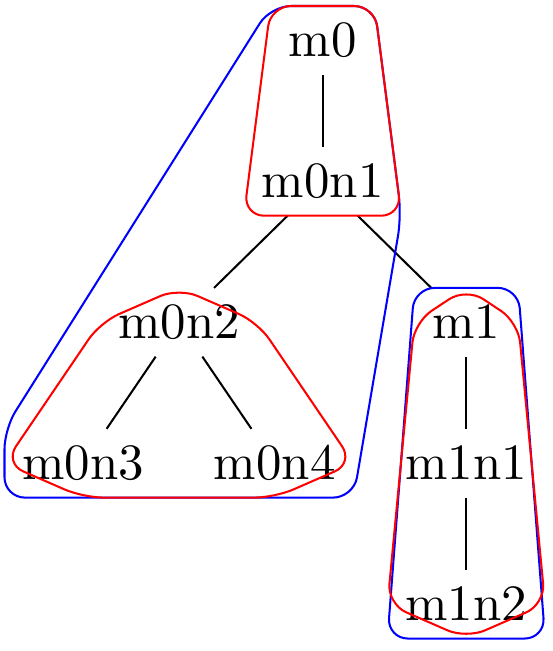
\includegraphics[scale=0.2]{F3C1Tree}
		\caption{Node order without Dummies}
		\label{factory:subim1}
	\end{subfigure}
	\begin{subfigure}{3cm}
		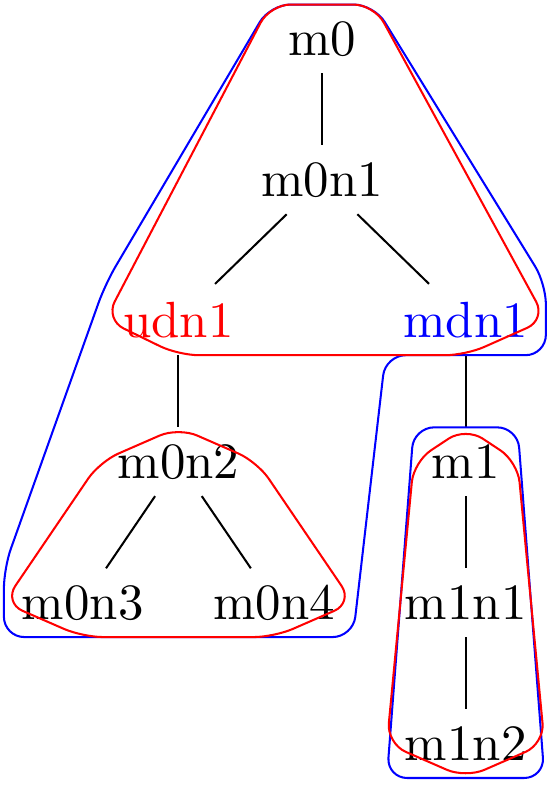
\includegraphics[scale=0.2]{F3C2Tree}
		\caption{Node order with Dummies}
		\label{factory:subim2}
	\end{subfigure}
	\begin{subfigure}{2.5cm}
		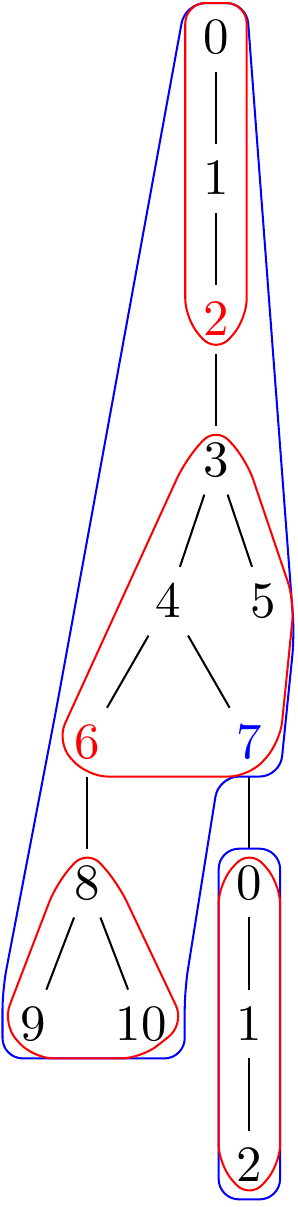
\includegraphics[scale=0.2]{F3C4Tree}
		\caption{Minitree specific node numbers}
		\label{factory:subim4}
	\end{subfigure}
	\begin{subfigure}{2.5cm}
		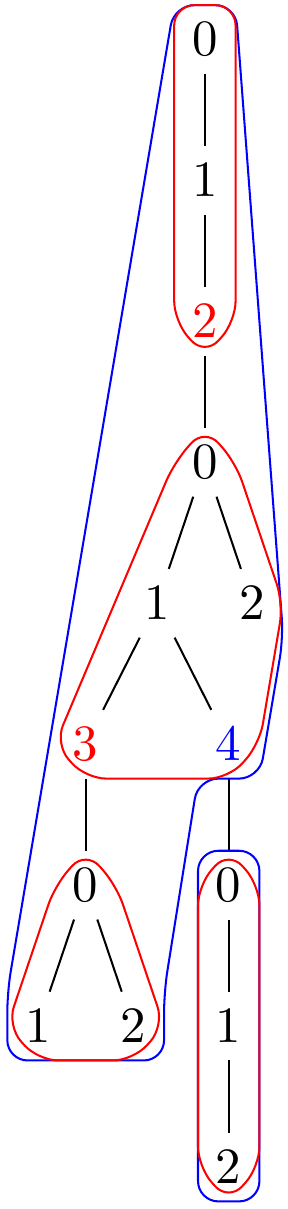
\includegraphics[scale=0.21]{F3C3Tree}
		\caption{Final Node numbers}
		\label{factory:subim3}
	\end{subfigure}

\caption{Special Cases regarding node order}
\label{factory:images4}
\end{figure}

The first issue originates from the handling of interconnections and the node numbering. While reading from an xml file retains the original node order from that xml, when adding dummies in the Unordered Tree class does not retain the original order of the nodes, especially when the Minidummy is located right after the Microdummy on the same level (\textit{Case a and b}). Therefore it becomes necessary to generate a consistent node numbering, which requires sorting the nodes within each tree. For this an \textit{enumerate} function is implemented that retains the original order from the xml file, and creates a consistent order for nodes within Mini and Microtrees, including added dummies.\\
Another issue is the identification of Minitree dummies within Microtrees (\textit{Case c and d}). Minitree dummies are originally identified by their node number respective to the Minitree as shown in figure \ref{factory:images4} (\textit{Case c}), where the Minidummy has the id of $7$, but the actual node id is $4$ (\textit{Case d}). However, due to the structure of Hypersuccinct nodes, it is necessary to translate the Minitree node numbers to Microtrees and Microtree node numbers. To solve this, we implemement a Microtree and node pointer for each Minitree dummy.

\subsection{Query Structures and Differences} \label{Query Structures and Differences}
Not all queries represented in \cite{farzanMunro} are implemented. This is in part due to the simplicity of this implementation, but also because the original paper is rather shortworded when describing the implementation of each query, or simply points towards other papers related to this topic, which were not part of the scope of this implementation.
Due to this there are some minor or notable differences to the paper at hand, which will be elaborated on in this section.

\subsubsection{Simple Queries} \label{Simple Queries}
As simple Queries we identify those queries that only require a single bitvector per level of abstraction. This means that these queries need one bitvector for values of each Minitree, one for each Microtree within the Minitrees and one for each lookup table entry.
As a result these queries all follow a similar structure, first handling single nodes, then generalizing the result to Microtrees and at last taking Minitrees into account to arrive at the correct result with an $O(1)$ time complexity.\\
These queries are:\\
\begin{itemize}
	\item[1)] \textit{getParent}
	\item[2)] \textit{degree}
	\item[3)] \textit{subtreeSize}
	\item[4)] \textit{depth}
	\item[5)] \textit{height}
	\item[6)] \textit{leftmostLeaf}
	\item[7)] \textit{rightmostLeaf}
	\item[8)] \textit{leafSize}
	\item[9)] \textit{levelSuccessor (Not implemented)}
	\item[10)] \textit{levelPredecessor (Not implemented)}
\end{itemize}
These queries are described as using one bitvector per abstraction in the paper. We therefore believe this implementation to be as described in the paper.\\
\textit{Degree} is specifically easy, since the degree of a given Microtree or Minitree root is just the size of their FIDs, making extra data bitvectors for \textit{degree} unnecessary on a Minitree and Microtree level. All other queries use their respective bitvectors to determine a result.\\
\textit{getParent} is not directly mentioned as a query in \cite{farzanMunro}. Instead, when describing the \textit{childRank} query, it is mentioned that we first have to identify the parent of the given node. We decided to make this into a separate helper query, anticipating to need this query for some other queries as well. As we already had the helper query, we also made a normal query out of it.
On Dummies:\\
These queries require to handle the dummy in query-specific ways. \textit{Depth} is the simplest query, only adding values from Minitree depth, Microtree depth and Node depth. These do already ignore dummies in their data, so this query does not require any dummy handling. \textit{Height} and \textit{subtreeSize} make use of the \textit{isDummyAncestor} helper queries to subtract the dummy from their calculations. \textit{Degree}, \textit{leftmostLeaf} and \textit{rightmostLeaf} check whether or not the current node is the dummy, and then move along its pointer. \textit{GetParent} simply checks if the result is a dummy, and then returns the parent of that dummy. This is still within $O(1)$, as there are at most two dummies (one Microdummy and one Minidummy) on top of one another.\\
Despite not being implemented, we can still make some observations about 
\textit{levelSuccessor} and \textit{levelPredecessor}. Both cannot use the FID to compute their results, as identifying a specific node in the FID is not possible in $O(1)$ (section \ref{The FID and identifying Trees}). We therefore believe that a bitvector pointing to either the FIDs position or directly to the successor/predecessor is necessary, therefore making both of these Simple Queries. For dummies both would use the same handling as getParent, as the value returned by the dummy is the correct one, whereas the dummy's child would be effectively one level too low.

\subsubsection{Rank Queries} \label{Rank Queries}
Rank Queries are all queries that return some sort of rank from the tree. These queries are more complicated than Simple Queries since they require more than one bitvector per abstraction.
Rank queries specifically need two bitvectors for the Minitree and Microtree abstractions, due to special cases.
They also require use of the FID to identify these special cases.\\
The Rank Queries are:\\
\begin{itemize}
	\item[1)] \textit{childRank}
	\item[2)] \textit{leafRank}
	\item[3)] \textit{nodeRank (Not implemented)}
\end{itemize}
The first issue comes up regarding the identification of the given node within an FID. Since we cannot identify the given node's position in the FID in constant time (section \ref{The FID and identifying Trees}), our implementation uses the FID to identify the special cases and then take information from additional bitvectors.

\begin{figure}[ht]
	\begin{subfigure}{2cm}
		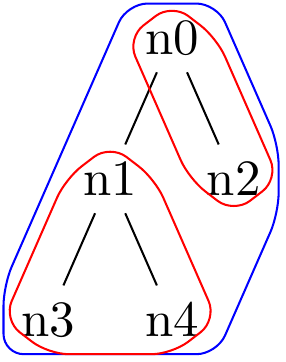
\includegraphics[scale=0.22]{F4C1Tree}
		\caption{Case 1}
		\label{rank:subim1}
	\end{subfigure}
	\begin{subfigure}{2cm}
		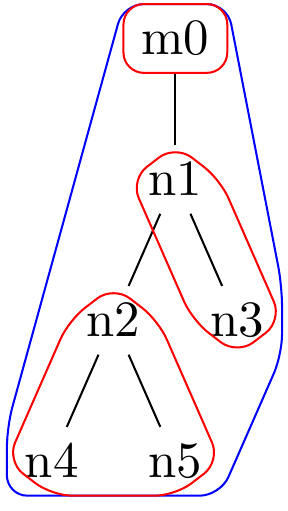
\includegraphics[scale=0.21]{F4C2Tree}
		\caption{Case 2}
		\label{rank:subim2}
	\end{subfigure}
	\begin{subfigure}{3cm}
		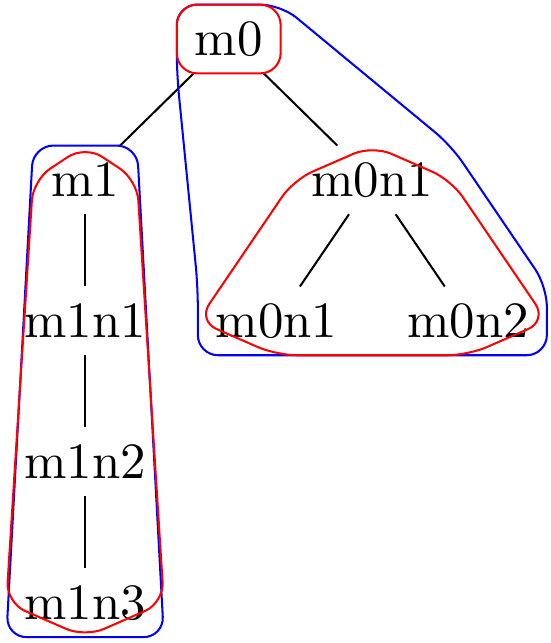
\includegraphics[scale=0.2]{F4C3Tree}
		\caption{Case 3}
		\label{rank:subim3}
	\end{subfigure}
	\begin{subfigure}{3cm}
		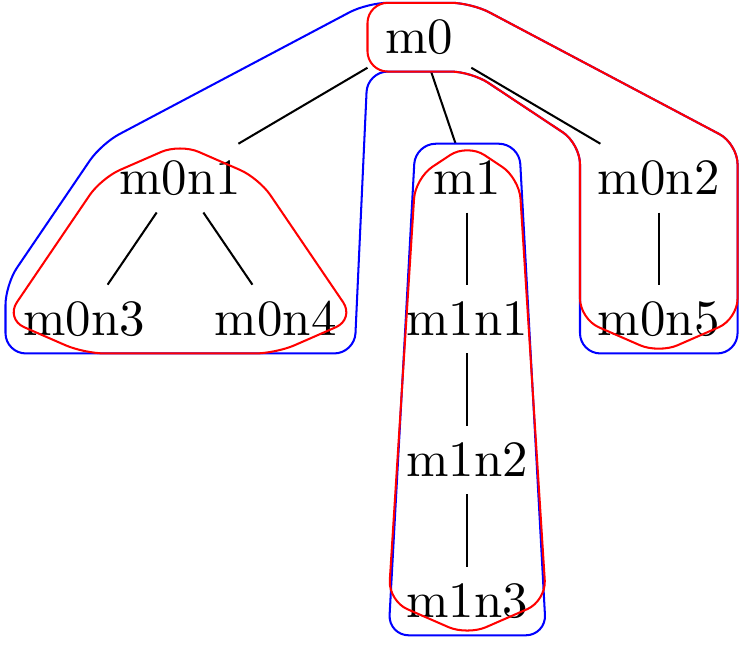
\includegraphics[scale=0.2]{F4C4Tree}
		\caption{Case 4}
		\label{rank:subim4}
	\end{subfigure}

\caption{4 Special Cases for Rank Queries}
\label{rank:images4}
\end{figure}

\begin{figure}[ht]
	\begin{tabular}{ |p{4cm}||p{1.5cm}|p{1.5cm}|p{1.5cm}|p{1.5cm}|  }
		 \hline
		 \multicolumn{5}{|c|}{Bitvectors} \\
		 \hline
		 Bitvector & Case 1 &Case 2&Case 3&Case 4\\
		 \hline
		 Minitree FID   & 1    & 1&   11 & 110\\
		 Minitree Typevector&   0  & 0   & 10 & 010\\
		 Microtree FID&11 &11&  irrelevant&irrelevant\\
		 Microtree Typevector&10& 10&  irrelevant&irrelevant\\
		 \hline
	\end{tabular}
\caption{FID and Typevector values for special cases}
\label{rank:table4}
\end{figure}

\textit{Case 1} and \textit{Case 2} describe a situation in which a higher indexed Microtree has a lower rank than the current Microtree. To resolve this, we introduce an extended rank bitvector which notes the rank of the first child of our current Microtree within the Minitree. This resolves this case on a data level, the second issue is to actually read the value of the extended bitvector in the right cases. This is where we differentiate between the two cases. If this problem appears at the Minitree root, we can identify this case by using the FID, resulting in \textit{Case 1}. If this problem appears further down in the Minitree we can compare values of Microtree and Node indices to identify \textit{Case 2}. \textit{Case 3} describes a similar issue regarding the Minitree. Again, a Minitree with a higher index has a lower rank than our current Minitree due to being a type 1 tree in the FID. This can also be identified with the FID. The three cases are mutually exclusive since they describe a similar issue.
\textit{Case 4} describes a tree of type 0 that is split by a tree of type 1 in between. This can be identified, since 0s in the FID must belong to the last type 0 tree, meaning after identifying the latest tree as being of type 1, one only needs to check if the index points to a 0 in the FID.\\
The structure of both queries is similar. First they calculate the result of only the node within the Microtree, using the values from the lookup table. Then, the result is generalized to a Microtree. Here, \textit{Case 2} is evaluated. At last, the result is generalized to the Minitree by analyzing key structures of the FID to identify \textit{Case 1}, or \textit{Case 3}. In \textit{childRank}, the special cases immediately return the value, as this query only needs to take into account the singular values of the parent FID. For \textit{leafRank}, a generalization to the entire tree is always necessary due to the result being sensitive to the entire tree topology.\\
Both implemented queries use \textit{getParentForQuery} as a helper query to identify the direct parent of the current node. These queries only check if the current node is a child of a dummy and if that is the case, the dummy is used instead, as the dummy is at the correct position to calculate the correct result.\\

\subsubsection{Child} \label{Child}
\textit{Child} is a more unique query. \textit{Child} is simpler than rank queries in principle, since the index provided by the query is directly related to an FID position, allowing an analysis of the node at that position in $O(1)$. It is important to note that identifying the correct child within the FID can point to a 0 value in the FID, and all issues for identifying nodes in the FID (Section \ref{The FID and identifying Trees}) apply here, making this query more complex.
This means that we need to identify Microtrees and nodes via the distance from the last $1$ within the respective FID of the Mini and Microtrees. To implement this, we first just identify the correct Minitree and reduce the remaining index by the position of that Minitree in the FID.
The process for identifying the Microtree is analogous to that, and at last we use the remaining index to select a specific node via the lookup table. If our starting node is already below the Minitree root, the part for identifying the right Minitree is skipped, same for Microtrees if we are below a Microtree root.
Dummy-nodes are skipped, both if the starting node is a dummy, in which case child of the direct pointer of the dummy is used instead, or if the result node is a dummy, in which case the direct pointer of the dummy is returned instead.\\
One thing we want to highlight is the identification of single nodes, below the Microtree. As \cite{farzanMunro} already describes, an Ancestor matrix is utilized for lookup table entries (Section \ref{Helper Queries}). Therefore, we first implemented a child matrix alongside it, to identify children within Microtrees. We were however not able to identify a way to implement this task in $O(1)$ without making use of \textit{Rank} and \textit{Select} queries, requiring us to implement a FID for the matrix, increasing the space complexity.

\subsubsection{Helper Queries} \label{Helper Queries}
Instead of being identified by their algorithmic structure, these queries are identified by the fact that they are used by other queries to compute their results.\\
These Helper Queries are:
\begin{itemize}
	\item[1)] \textit{isDummyAncestorWithinMiniTree}
	\item[2)] \textit{isDummyAncestorWithinMicroTree}
	\item[3)] \textit{getParentForQuery}
\end{itemize}
Their implementation is similar to the implementation of Simple Queries.\\
\textit{GetParentForQuery} is a special version of \textit{getParent} that excludes handling for dummy nodes. This is necessary to identify special dummy cases in the queries that use this Helper Query (such as \textit{child}).
The \textit{isDummyAncestor} helper queries identify if a given node is an ancestor of a Minidummy or a Microdummy respectively. \textit{IsDummyAncestorWithinMiniTree} has a similar structure to the simple queries, first using specific bitvector data that contains if the Microtree root is an ancestor of the dummy, then if the specific node is the ancestor. \textit{IsDummyAncestorWithinMicroTree} is even simpler, only needing to determine the answer for specific nodes. Both queries are necessary to evaluate an entire tree structure in $O(1)$, since they prevent the necessity to analyze every node on the structure individually, which would not be possible in constant time. These queries utilize the lookup table's ancestor matrix as described by \cite{farzanMunro}.

\subsubsection{Other Queries / Not implemented Queries} \label{Other Queries / Not implemented Queries}
The following queries are not implemented and are not similar enough to already implemented queries to use those as a template. We briefly describe our issues with those queries.
\begin{itemize}
	\item[1)] \textit{nodeSelect (Not implemented)}
	\item[2)] \textit{levelAncestor (Not implemented)}
	\item[3)] \textit{lowestCommonAncestor (Not implemented)}
	\item[4)] \textit{distance (Not implemented)}
	\item[5)] \textit{levelLeftmostNode (Not implemented)}
	\item[6)] \textit{levelRightmostNode (Not implemented)}
\end{itemize}
Moving multiple levels is not trivial with our encoding. Since this is supposed to work in $O(1)$ time we are not sure how to implement a level based query. Moving up one level at a time is not constant in total, but adding one bitvector per level for each Microtree violates the space complexity requirement. This issue applies to queries 2) to 6).\\
\textit{NodeSelect} has to call to a full mapping that orders all nodes with a single index, which is not how Hypersuccinct nodes are represented. Again, saving such a map for each Microtree and Minitree violates our space complexity requirement, but computing it violates the time complexity requirement.

\subsection{Other Classes} \label{Other Classes}
There are a variety of other classes within the library that contribute to the functionality of our library.
\begin{itemize}
	\item[1)] \textit{Bitvector Utils}\\
			Bitvector Utils is a basic class that provides utility functions for Bitvectors. Its main function is to typecast Bitvectors to Integers and back, which is possible in $O(1)$ due to the limited size of Integers. (i.e. \textit{uint32\_t} has a maximum of $32$ bits.)
	\item[2)] \textit{HST Output}\\
			The HyperSuccinctTree Output class provides functions for writing and reading a Hypersuccinct Tree class. Therefore this class handles writing Hypersuccinct Trees to Files or reading Hypersuccinct Trees from Files. It also supports writing the entire tree into the console.
	\item[3)] \textit{Unordered Tree}\\
			Unordered Tree is our basic tree implementation, to which an xml tree is parsed. Unordered Trees are then used to create Hypersuccinct Trees. The tree does not guarantee to retain the correct order of nodes when adding nodes, however it does retain the order of nodes read from an xml tree, which is what it is used for.
	\item[4)] \textit{Precomputed Function and Cached Function}\\
			These two classes are used to improve the performance of the \textit{HypersuccinctTreeFactory}'s \textit{create} function by either completely precomputing values for queries within the Unordered Tree, or by caching already calculated values.
	\item[5)] \textit{XML Reader}\\
			This class reads the actual xml file and creates an Unordered Tree from it, retaining the correct node order.
	\item[6)] \textit{Farzan Munro}\\
			The Farzan Munro class implements the algorithm as presented in \cite{farzanMunro}. It therefore implements \textit{decomopose} and \textit{greedilyPack}. It also orders the created Tree afterwards to guarantee a consistent order within the hypersuccinct tree.
\end{itemize}

\subsection{Runtime tests} \label{Runtime tests}
In order to test if our code fulfills the aforementioned boundaries of time we implemented several tests. Each of these tests first encodes a xml-file to a Hypersuccinct Tree, then runs several queries on up to 1000 nodes of the tree and records the time it takes to run for each run query. With these records we can show how fast the calls to each query where executed and calculate averages or boxplots. This, however, does not take into account the speed of the machine or other randomness effects related to the execution of the code on our computers.\\

\section{Complexity Benchmarks} \label{Complexity Benchmarks}
In this section we discuss some specific design decisions and shortcomings, and how they affect the performance of our hypersuccinct encoding.
\subsection{Huffman encoding}
\begin{figure}[h]
	\begin{tabular}{ |p{4.5cm}||p{2cm}|p{2cm}|p{4cm}|  }
		 \hline
		 Tree Name & Normal &Huffman &Huffman + Lookuptable\\
		 \hline
		 TreeNath.xml 		&52    		&23 		&24 		\\
		 TreeNath2.xml		&484  		&256   	&266 		\\
		 TreeNath3.xml		&5196 	&2695		&2706		\\
		 TreeNath4.xml		&53369	&31709	&31732	\\
		 TreeNath5.xml		&583289	&345005	&345029	\\
		 DBLP.xml			&3690039	&593804	&593842	\\
		 XMark2.xml			&2004196	&831572	&831627	\\
		 \hline
	\end{tabular}
\caption{Space for normal encoding and huffman encoding in byte}
\label{huff:table1}
\end{figure}
Our tree offers two types of encoding for Microtrees. The first option encodes trees according to \cite{farzanMunro}, and uses the Microtree's balanced parenthesis representation, while the other utilizes a huffman encoding for the Microtrees. For that, the Microtrees use their respective huffman codes in the representation, while their corresponding lookup table entries contain the balanced parenthesis representation for each code.\\
The huffman encoding has no impact on query performance, as finding a corresponding lookup table entry for a huffman code is possible in $O(1)$. Encoding trees with huffman has a significant impact on the space necessary for the Microtree encoding since the balanced parenthesis representation needs $2n$ many bits for a tree of size $n$, while huffman codes are more efficient (See Section \ref{Space Complexity}).

\subsection{Factory Complexity} \label{Factory Complexity}
The encoding process in \textit{create} is obviously not possible in $O(1)$, due to the Farzan-Munro algorithm itself being more complex, and the current implementation amounts to roughly $O(n^{3})$. Despite that we put significant effort into increasing the performance of the encoding process. The \textit{create} was evaluated in four separate options, whether or not to use huffman encoding, and whether or not to generate query data.\\
In addition to that we also analyzed the runtime of \textit{writeToFile} and \textit{readFromFile}.
\begin{figure}[H]
	\begin{tabular}{ |p{3cm}||p{2,5cm}|p{2,5cm}|p{2,5cm}| }
		 \hline
		 Tree Name & Create & Write File &Read File\\
		 \hline
		 TreeNath.xml   & 00:00:00.056    & 00:00:00.003 &   00:00:00.026 \\
		 TreeNath2.xml&   00:00:00.081  & 00:00:00.003   & 00:00:00.023 \\
		 TreeNath3.xml&00:00:00.209 &00:00:00.033&  00:00:00.073\\
		 TreeNath4.xml&00:00:02.266& 00:00:00.308&  00:00:00.510\\
		 TreeNath5.xml&00:00:36.357&00:00:03.558&00:00:06.413\\
		 XMark2.xml&00:00:58.005&00:00:07.645&00:00:20.307\\
		 DBLP.xml&00:04:52.509&00:00:10.888&00:00:30.038\\
		 \hline
	\end{tabular}
\caption{Average runtimes for create, writing and reading files for specific trees}
\label{complexFac:table1}
\end{figure}
\begin{figure}[H]
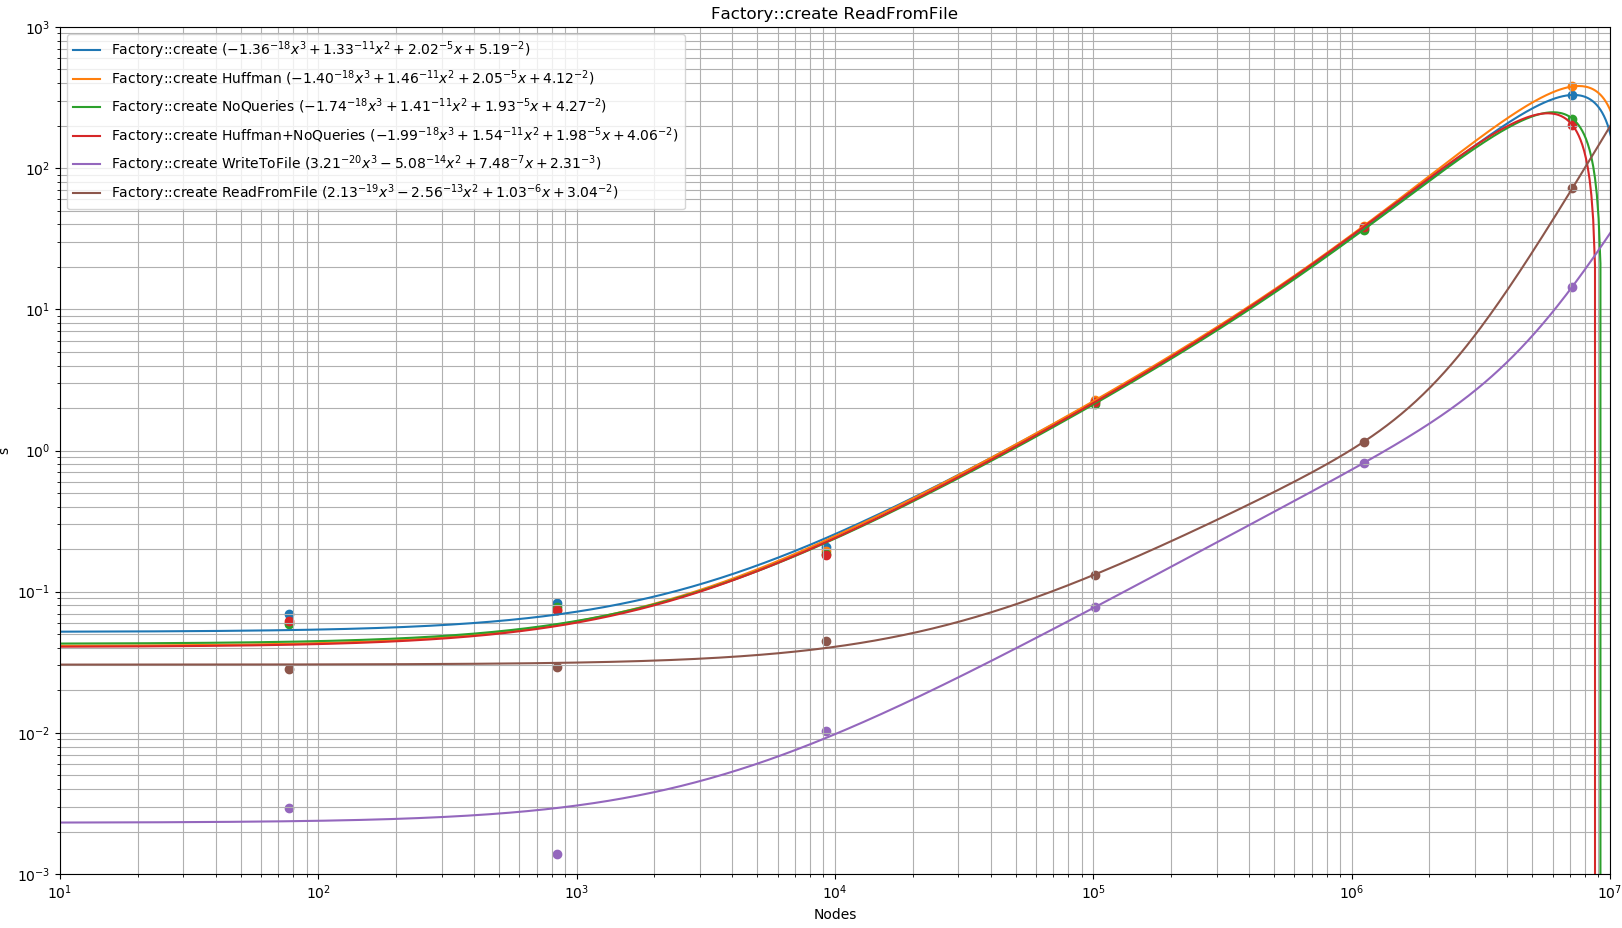
\includegraphics[scale=0.3]{file_compare_cut}
\caption{Runtime of \textit{create}}
\label{complexFac:image1}
\end{figure}

\subsection{Query Complexity} \label{Query Complexity}
For query runtime tests we used \textit{DBLP}, which is a large, flat tree, and \textit{treeNath1-5}, which are trees of growing size and depth. The records we got from these tests show that queries on Hypersuccint Trees of vastly different size are still in the same magnitude of execution time. The longer execution times of larger trees compared to smaller trees can be accounted longer access times related to caching and hardware behaviour. The code itself maintains it's $O(1)$ execute time magnitude.\\
The queries provided by the hypersuccinct tree are implemented in $O(1)$, as specified in
\cite{farzanMunro}. As shown in Figure \ref{complexQue:image2} all queries except \textit{child} have an average runtime of well below $100 \mu s$. When it comes to \textit{child} when comparing between our different trees, the average runtime of \textit{child} increases with an increased 
\begin{figure}[H]
\includegraphics[scale=0.3]{treeNath3_Queries}
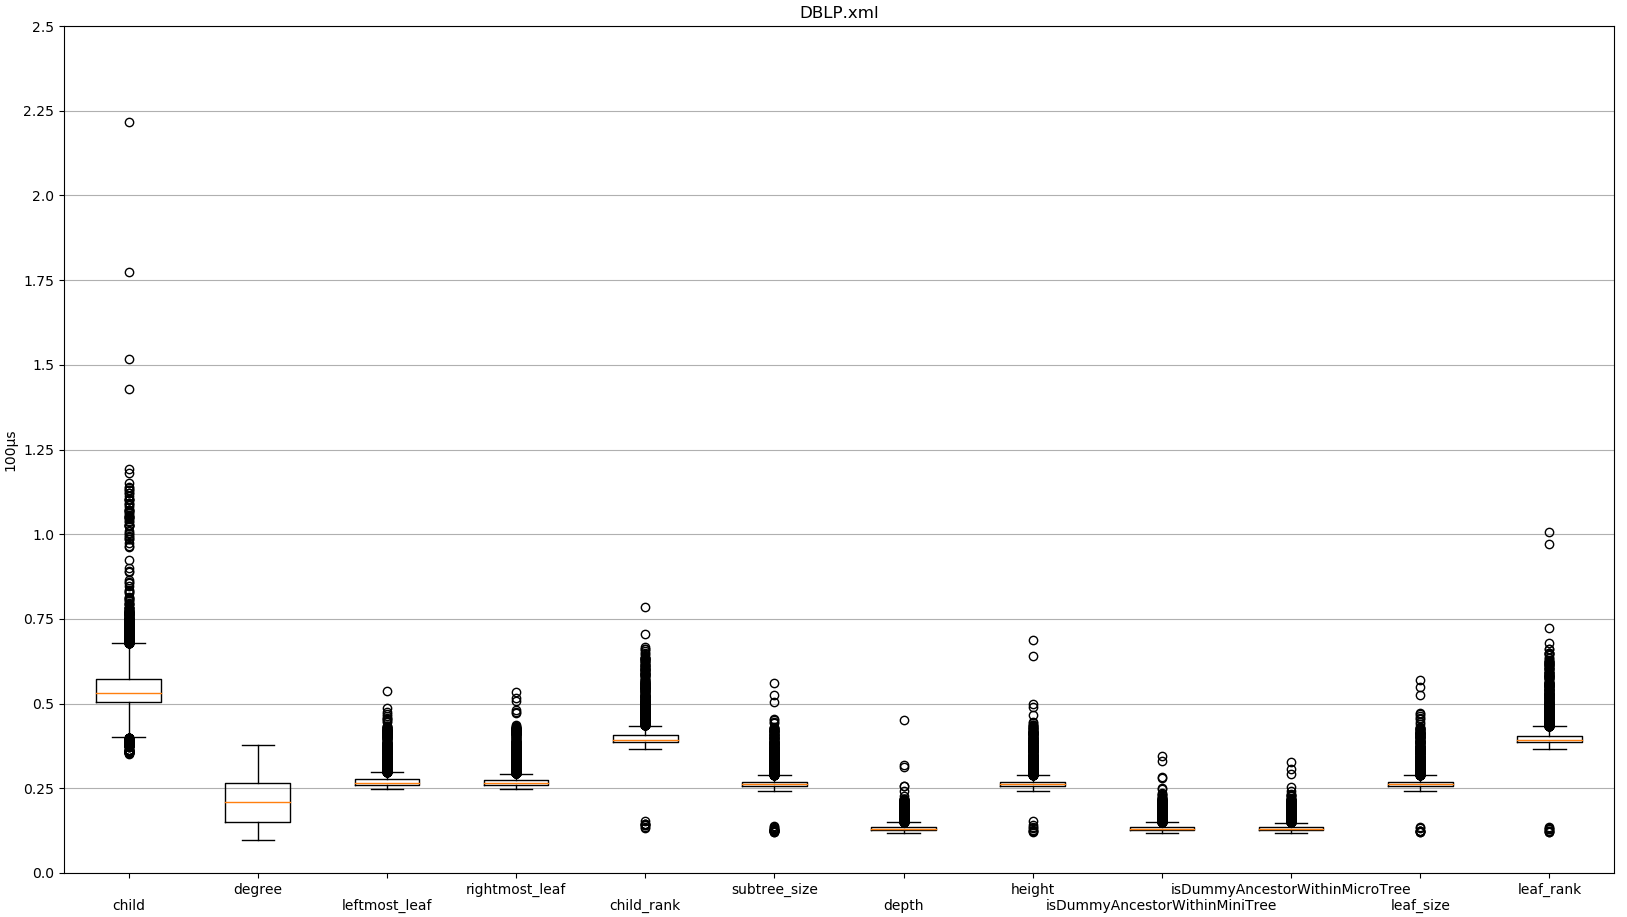
\includegraphics[scale=0.3]{DBLP_Queries}
\caption{Runtime of implemented queries}
\label{complexQue:image2}
\end{figure}
amount of nodes. However, when analyzing our code, we were not able to find a section that would violate the $O(1)$ complexity requirement, not in our query implementation nor in the \textit{succinct\_bv} library. With some testing we determined that the increase in runtime stems from the basic function \textit{getMinitree}, which returns the Minitree for a given index, which is important for our evalutation, as hypersuccinct nodes save their Minitree as an integer (see Section \ref{The Hypersuccinct Tree Class}). Since this function simply calls the [] operator of \textit{std::vector}, which per the C++ definition is $O(1)$. We therefore argue that our code maintains constant time.

\subsection{Space Complexity} \label{Space Complexity}
In this section we discuss the space complexity of our hypersuccinct tree implementation. For that  let $n$ be the size of the entire tree, $m_{fm}$ be the calculated Minitree size of $\lceil \log^{2} n \rceil$, and $\mu_{fm}$ be the calculated Microtree size of $\lceil \frac{\log n}{8} \rceil$. Let this tree have $l$ many Minitrees $M$, and let $m_{j}$ be the actual size of the j-th Minitree.\\

We assume that our implementation of the Farzan Munro algorithm, consisting of \textit{decompose} and \textit{greedilyPack}, is correct, and therefore fulfills the requirements for Theorem 1 from \cite{farzanMunro}.

\subsubsection{Amount of Trees} \label{Amount of Trees}
Per Theorem 1 from \cite{farzanMunro} there are $O(\frac{n}{\log ^{2} n})$ many Minitrees, and $O(\frac{n}{\log {n}})$ many Microtrees in the entire tree.\\
In any Minitree $M_{j}$, since their maximum size is $2 \cdot m_{fm} = 2 \cdot \lceil \log^{2} n \rceil$, and the amount of Microtrees follows $\Theta (\frac{m_{j}}{\mu_{fm}})$, the amount of Microtrees in each Minitree is:
$$O \left( \frac{2 \cdot m_{fm}}{\Theta \left( \frac{m_{j}}{\mu_{fm}}\right) }\right) $$
$$\leq O \left( \frac{2 \cdot m_{fm} \cdot \mu_{fm}}{m_{fm}} \right)$$
$$ = O(\mu_fm) = O \left( \lceil \frac{\log n}{8} \rceil \right) = O(\log n)$$\\

The amount of Lookuptable entries depends on the amount of unlabeled ordered trees of a size less than $2 \cdot \mu_fm$. This amount is described by the Catalan Numbers $Ca(n)$ where for a given amount of nodes $n$, the amount of trees with this size is described by $Ca(n-1)$. We therefore have a sum of all possible trees with a smaller or equal size to $2\cdot \mu_{fm}$:
$$\sum_{v=1}^{2\mu_{fm}} Ca(v-1)$$
$$\in O\left( \sum_{v=1}^{2\mu_{fm}} Ca(v-1) \right)$$
$$\in O\left( \sum_{v=1}^{2\mu_{fm}} 4^{v} \right) \in O \left( 4^{\frac{\log n}{4}} \right)$$
$$\in O(\sqrt{n})$$\\

Since there can only be one dummy in each tree per level of abstraction, dummies contribute the same complexity as the amount of trees, so there are $O(\frac{n}{\log ^{2} n})$ Minidummies, $O(\frac{n}{\log {n}})$ Microdummies in total, and $O(\log n)$ many Microdummies in each Minitree.\\
Dummy pointers for Minitrees take up $O( \log \log n)$ many bits per dummy per pointer. Since there are $O(\frac{n}{\log ^{2} n})$ many Minidummies, they take a total of $O(\frac{n}{\log ^{2} n} \cdot \log \log n)$. Analogously, for Microtrees, the dummies take $O(\frac{n}{\log {n}} \log \log n)$ bits of space.

\subsubsection{Encoding Complexity} \label{Encoding Complexity}
We can now use the above information to decide on the complexity of our Microtree encoding.\\

For the normal Microtree encoding we use balanced parenthesis forms, which take $2 \cdot \mu_{i}$ many bits for a Microtree $P_{i}$ of size $\mu_{i}$. We know there are $O(\frac{n}{\log {n}})$ many Microtrees in total, and their nodes sum up to $n$, and they have $O(\frac{n}{\log {n}})$ many possible additional shared roots, as well as $O(\frac{n}{\log {n}})$ many additional Microdummies, and $O(\frac{n}{\log ^{2} n})$ many additional Minitree nodes.
This leads to a total of $2n + O(\frac{n}{\log {n}}) + O(\frac{n}{\log {n}}) + O(\frac{n}{\log ^{2} n})$ many bits for our Microtree encoding.
For huffman encoding, \cite{universalSuccinct} proved that this encoding takes $\leq 2n$ bits to encode all nodes, and is therefore more efficient.

FIDs have a complexity of $f + O\left( \frac{f \log \log f}{\log f} \right)$, for a base vector of size $f$. Now assume a tree that has only a depth of $1$, with one root, and all other nodes being direct children of the root. In this worst possible case, our Minitree FIDs hold all nodes except on, the root of the tree, and therefore make up $n-1$ bits in total. In that case, since there are $m_{fm}$ many Minitrees, for each Minitree, their Microtree FIDs hold $\frac{n}{\log ^{2}n}$ many bits each, which sums up to $n-1$ again.\\
Therefore in total, the FIDs take $2n + O\left( \frac{n \log \log n}{\log n} \right) \in 2n + o(n)$ many bits.

The Typevectors save one bit for each unique tree from their related FID. Since all trees, that are not the tree root or below a dummy, have two FID entries, we have a total of $O(2 \cdot \frac{n}{\mu_{fm}})$ bits for the Microtrees and $O(2 \cdot \frac{n}{m_{fm}})$ bits for the Minitrees so there are $O(\frac{n}{\log n})$ bits in total. Since Typevectors also use \textit{Rank} and \textit{Select}, we have a total complexity of:
$$O \left( \frac{n}{\log n}\right) + O\left( \frac{ O \left( \frac{n}{\log n}\right) \log \log O \left( \frac{n}{\log n}\right)}{\log O \left( \frac{n}{\log n}\right)} \right)$$
$$\leq O \left( \frac{n}{\log n}\right) + o(n)$$
$$\in o(n)$$

In the Minitree struct we save query data pertaining to the current Minitree and to all its Microtrees. Query data for each Minitree is $O(1)$ per tree, and therefore amounts to $O(\frac{n}{\log ^{2} n})$ in total, for each Microtree it is also $O(1)$, and in total $O(\frac{n}{\log {n}})$.

In the lookuptable entries we save query data for each node. For a lookuptable entry of size $\mu_{h}$, most queries save $\mu_{h}$ bits of data. However, the ancestor matrix saves $\mu_{h}^{2}$ many bits. When we take into account the amount of entries we get:
$$\sum_{v=1}^{2\mu_{fm}} \left( Ca(v-1) \cdot v^{2} \right)$$
$$\in O\left( \sum_{v=1}^{2\mu_{fm}} Ca(v-1) \cdot v^{2} \right)$$
$$\in O\left( \sum_{v=1}^{2\mu_{fm}} 4^{v} \cdot v^{2} \right)$$
$$\in O \left( 4^{\frac{\log n}{4}} \cdot \left( \frac{\log n}{4} \right)^{2} \right)$$
$$\in O(\sqrt{n} * (\log n)^{2})$$
$$\leq o(n)$$ %By the way: x and root(x)*log(x)^2 intersect at 2^16.

\subsubsection{Total Space Complexity} \label{Total Space Complexity}
In total, for a tree of size $n$, there are $O(\frac{n}{\log ^{2} n})$ many Minitrees, and $O(\frac{n}{\log {n}})$ many Microtrees in the entire tree. There are also $O(\sqrt{n})$ many lookuptable entries in the tree. The Microtree encoding takes $2n + o(n)$ many bits, this is also the case for the FIDs, while Typevectors take $o(n)$ many bits. The dummies and dummy pointers both take $o(n)$ many bits, as do all queries.\\
This all adds up to a total complexity of $4n + o(n)$.


\subsection{Space Complexity concessions} \label{Space Complexity concessions}
Our encoding does not meet the provided theoretical complexity of $2n + o(n)$. Additionally, the implementation adds a very large constant factor to the encoding as well, which further increases the space necessary for our tree encoding. We identify the following reasons for this discrepancy:\\
\begin{itemize}
	\item[1)] The \textit{succinct\_bv} library does not meet the perfect space complexity from \cite{succinctBV} of $\log \left( \!\begin{array}{c} n \\ r \end{array}\! \right) + O\left( \frac{n \log \log n}{\log n} \right)$, and instead has a complexity of $n + O\left( \frac{n \log \log n}{\log n} \right)$ for a bitvector of size $n$. This is the reason for our inceased space complexity. Using the more optimal implementation, our space complexity would drop to $2n + o(n)$, since to other $2n$ hail from the FIDs, which are affected by this.
	\item[2)] The implementation of \textit{Bitvector} in $C++$ saves its data as \textit{uint32\_t}, which is always 32 bits long. This is a massive waste of space, since most values are much smaller than 32 bits. This is not an issue for the encoded file, only for the program itself.
	\item[3)] While the complexity of query data in the lookuptable entries is below $o(n)$ technically, it only takes less than $n$ bits for values over $2^{16}$, which is only possible for a total tree size of $4 \cdot 2^{(2^{16})}$.
\end{itemize}
For \textit{1)}, it is necessary to either use a library that offers the improved complexity, or to improve the current library.\\
For \textit{2)}, we believe it to be possible to save the entire hypersuccinct tree in a single bitvector. It should be possible to use pointers to access different parts of this bitvector in $O(1)$ using a variable cell array, as described in \cite{universalSuccinct}.\\
For \textit{3)}, reducing the complexity of the query data in the lookuptable is necessary.

\section{Conclusion} \label{Conclusion}
In this work we demonstrated that an implementation of a hypersuccinct tree is not only possible, but also usable in real-world scenarios. Both a theoretical analysis and a practical evaluation of a test service have shown that the space-efficiency of our implementation is sufficiently high, and follows the instructions presented in \cite{farzanMunro}. We were also able to implement queries in a constant time.\\
Also noteworthy is the effect of the application of the Huffman encoding for microtree-representation, which further improves the space-complexity by a significant amount.\\
Further work could be done by implementing some missing complex and underspecified queries. Additional optimization potential regarding the memory-footprint of our library also exists (e.g. merging bitvectors together).\\
Nonetheless, our example applications show that our implementation is more than sufficient to process common Use-Cases, such as loading a tree from an existing file, parsing another tree format to a hypersuccinct tree, visualizing the tree and queries and saving the results back to a file.

\pagebreak
\section{Data}  \label{Data}
All trees can be found in the resources folder of our project on Github, on \href{https://github.com/ChristopherPack/Projektgruppe\_Hypersuccint\_Trees}{https://github.com/ChristopherPack/Projektgruppe\_Hypersuccint\_Trees}, or on \href{http://xmlcompbench.sourceforge.net/Dataset.html}{http://xmlcompbench.sourceforge.net/Dataset.html}.
\subsection{Used xml tree files}
\begin{figure}[H]
	\begin{tabular}{ |p{3cm}||p{2,5cm}||p{2,5cm}| }
		 \hline
		 Tree Name & Size & Depth\\
		 \hline
		 TreeNath.xml   &77 & 8\\
		 TreeNath2.xml&  837 & 31\\
		 TreeNath3.xml&9197 & 119\\
		 TreeNath4.xml&101157 & 228\\
		 TreeNath5.xml&1112717 & 351\\
		 XMark2.xml&3603803 & 12\\
		 DBLP.xml&7146530 & 6\\
		 \hline
	\end{tabular}
\caption{sizes of our xml trees}
\label{data:table1}
\end{figure}
\subsection{Additional Huffman comparisons}
\begin{figure}[H]
	\begin{tabular}{ |p{4.5cm}||p{2cm}|p{2cm}|p{4cm}|  }
		 \hline
		 Tree Name & Normal &Huffman &Huffman + Lookuptable\\
		 \hline
		 TreeNath.xml 		&52    		&23 		&24 		\\
		 TreeNath2.xml		&484  		&256   	&266 		\\
		 TreeNath3.xml		&5196 	&2695		&2706		\\
		 TreeNath4.xml		&53369	&31709	&31732	\\
		 TreeNath5.xml		&583289	&345005	&345029	\\
		 DBLP.xml			&3690039	&593804	&593842	\\
		 EnWikiNew.xml		&208736	&62920	&62931	\\
		 EnWikiQuote.xml		&135452	&42033	&42044	\\
		 EnWikiVersity.xml		&254354	&72622	&72633	\\
		 EnWikiTionary.xml		&4257416	&1136761	&1136772	\\
		 EXI-Array.xml		&110700	&23611	&23629	\\
		 EXI-factbook.xml		&34671	&8764		&8769		\\
		 EXI-GeogCoord.xml	&13		&7		&8		\\
		 EXI-Invoice.xml		&9093		&3063		&3068		\\
		 EXI-Telecomp.xml		&101223	&50656	&50680	\\
		 EXI-weblog.xml		&58101	&12446	&12451	\\
		 Lineitem.xml			&638109	&119099	&119104	\\
		 Mondial.xml			&13523	&3838		&3843		\\
		 Nasa.xml			&238346	&101229	&101273	\\
		 Random-R1.xml		&128122	&74701	&74791	\\
		 Random-R3.xml		&871406	&198523	&198593	\\
		 Shakespeare.xml		&98521	&26097	&260123	\\
		 SwissProt.xml		&1745940	&404339	&404364	\\
		 Treebank.xml		&1274173	&752081	&752166	\\
		 USHouse.xml		&3628		&1151		&1161		\\
		 XBench-DCSD-Normal.xml	&1132157	&455538	&455556	\\
		 XBench-DCSD-Small.xml	&113979	&46120	&46137	\\
		 XBench-TCSD-Normal.xml	&1543295	&563397	&563422	\\
		 XBench-TCSD-Small.xml	&159204	&58507	&58532	\\
		 XMark1.xml			&95623	&42484	&42521	\\
		 XMark2.xml			&2004196	&831572	&831627	\\
		 \hline
	\end{tabular}
\caption{Space for normal encoding and huffman encoding in byte}
\label{huffData:table1}
\end{figure}

\pagebreak
\bibliographystyle{IEEEtran}
\bibliography{references}

\end{document}
